
\documentclass{beamer}
\usecolortheme{dove}
\setbeamertemplate{navigation symbols}{}
\usepackage{amsmath,amssymb,amsfonts,amsthm, multicol, subfigure, color}
\usepackage{bm}
\usepackage{graphicx}
\usepackage{tabularx}
\usepackage{booktabs}
\usepackage{hyperref}
\usepackage{pdfpages}
\usepackage{xcolor}
\definecolor{seagreen}{RGB}{46, 139, 87}
\def\independenT#1#2{\mathrel{\rlap{$#1#2$}\mkern2mu{#1#2}}}
\newcommand\indep{\protect\mathpalette{\protect\independenT}{\perp}}
\def\log{\text{log}}
\newcommand\logit{\text{logit}}
\newcommand\iid{\stackrel{\text{iid}}{\sim}}
\newcommand\E{\text{E}}
\newcommand\V{\text{V}}
\renewcommand\P{\text{P}}
\newcommand{\Cov}{\text{Cov}}
\newcommand{\Cor}{\text{Cor}}
\newcommand\doop{\texttt{do}}
\usepackage{stackrel}
\usepackage{tikz}
\usetikzlibrary{arrows,shapes.arrows,positioning,shapes,patterns,calc}
\newcommand\slideref[1]{\vskip .1cm \tiny \textcolor{gray}{{#1}}}
\newcommand\red[1]{\color{red}#1}
\newcommand\blue[1]{\color{blue}#1}
\newcommand\gray[1]{\color{gray}#1}
\newcommand\seagreen[1]{\color{seagreen}#1}
\newcommand\purple[1]{\color{purple}#1}
\newcommand\orange[1]{\color{orange}#1}
\newcommand\black[1]{\color{black}#1}
\newcommand\white[1]{\color{white}#1}
\newcommand\teal[1]{\color{teal}#1}
\newcommand\magenta[1]{\color{magenta}#1}
\newcommand\Fuchsia[1]{\color{Fuchsia}#1}
\newcommand\BlueGreen[1]{\color{BlueGreen}#1}
\newcommand\bblue[1]{\textcolor{blue}{\textbf{#1}}}
\newcommand\bred[1]{\textcolor{red}{\textbf{#1}}}
\newcommand\bgray[1]{\textcolor{gray}{\textbf{#1}}}
\newcommand\bgreen[1]{\textcolor{seagreen}{\textbf{#1}}}
\newcommand\bref[2]{\href{#1}{\color{blue}{#2}}}
\colorlet{lightgray}{gray!40}
\pgfdeclarelayer{bg}    % declare background layer for tikz
\pgfsetlayers{bg,main} % order layers for tikz
\newcommand\mycite[1]{\begin{scriptsize}\textcolor{darkgray}{(#1)}\end{scriptsize}}
\newcommand{\tcframe}{\frame{
%\small{
\only<1|handout:0>{\tableofcontents}
\only<2|handout:1>{\tableofcontents[currentsubsection]}}
%}
}

\usepackage[round]{natbib}
\bibliographystyle{humannat-mod}
\setbeamertemplate{enumerate items}[default]
\usepackage{mathtools}
\usepackage{ulem}

% Need to add examples

\newcommand{\goalsframe}{\begin{frame}{Learning goals for today}
\begin{enumerate}
\item define causal estimands
\item make causal assumptions with Directed Acyclic Graphs
\item estimate with inverse probability weights
\begin{itemize}
\item in one period
\item in two periods
\end{itemize}
\item estimate with a marginal structural model
\end{enumerate} \vskip .2in
\end{frame}}

\title{Marginal Structural Models}
\author{Ian Lundberg}
\date{17 Nov 2023}

\begin{document}

\maketitle

\goalsframe

\begin{frame}{Running example}

%What is the cumulative effect of studying $\vec{A}$\\
%on a student's final exam score? \vskip .05in
\begin{itemize}
\item at time 1,
\begin{itemize}
\item a student receives a midterm test score $X_1$
\item they decide whether to study more $A_1$
\end{itemize}
\item at time 2,
\begin{itemize}
\item a student receives a midterm test score $X_2$
\item they decide whether to study more $A_2$
\end{itemize}
\item they get a final exam score $Y$
\end{itemize}

\begin{center}
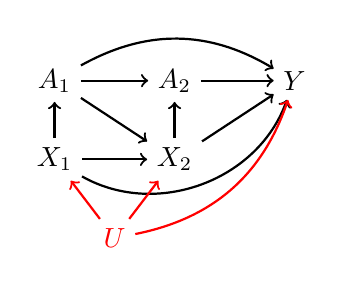
\begin{tikzpicture}[x = .6in]
\node (y) at (2,0) {$Y$};
\node[red] (u) at (.5,-2) {$U$};
\node (l0) at (0,-1) {$X_1$};
\node (a0) at (0,0) {$A_1$};
\node (l1) at (1,-1) {$X_2$};
\draw[->, thick] (l0) -- (a0);
\draw[->, thick] (l0) to[bend right = 50] (y);
\draw[->, thick] (a0) to[bend left] (y);
\node (a1) at (1,0) {$A_2$};
\draw[->, thick] (a0) -- (a1);
\draw[->, thick] (l0) -- (l1);
\draw[->, thick] (a0) -- (l1);
\draw[->, thick] (l1) -- (a1);
\draw[->, thick] (l1) -- (y);
\draw[->, thick] (a1) -- (y);
\draw[->, thick, red] (u) -- (l0);
\draw[->, thick, red] (u) -- (l1);
\draw[->, thick, red] (u) to[bend right] (y);
\end{tikzpicture}
\end{center}

\end{frame}

\begin{frame}{Defining causal effects}{Effect of studying at time 2}
Expected outcome $\E(Y^{a_2})$ if assigned\\to the value $a_2$ for studying at time 2  \vskip .2in
\begin{tabular}{ccc}
Student & $Y^{a_2=0}$ & $Y^{a_2=1}$ \\
\hline
1 & 80 & 95 \\
2 & 70 & 95 \\
3 & 90 & 90 \\
\vdots & \vdots & \vdots
\end{tabular}
\end{frame}
\begin{frame}{Defining causal effects}{Effect of studying at time 2}
Expected outcome $\E(Y^{a_2})$ if assigned\\to the value $a_2$ for studying at time 2  \vskip .2in
\begin{tabular}{ccc}
Student & $Y^{a_2=0}$ & $Y^{a_2=1}$ \\
\hline
1 & 80 & ? \\
2 & 70 & ? \\
3 & ? & 90 \\
\vdots & \vdots & \vdots
\end{tabular}
\end{frame}

\begin{frame}{Defining causal effects}{Effect of studying at time 1 and 2}
Expected outcome $\E(Y^{a_1,a_2})$ if assigned\\to the value $(a_1,a_2)$ for studying at time 1 and time 2  \vskip .2in
\begin{tabular}{ccccc}
Student & $Y^{a_1=0,a_2=0}$ & $Y^{a_1=0,a_2=1}$ & $Y^{a_1=1,a_2=0}$ & $Y^{a_1=1,a_2=1}$ \\
\hline
1 & 70 & 80 & 75 & 90 \\
2 & 80 & 95  & 80 & 95\\
3 & 90 & 90 & 90 & 90 \\
\vdots & \vdots & \vdots & \vdots & \vdots
\end{tabular}
\end{frame}
\begin{frame}{Defining causal effects}{Effect of studying at time 1 and 2}
Expected outcome $\E(Y^{a_1,a_2})$ if assigned\\to the value $(a_1,a_2)$ for studying at time 1 and time 2  \vskip .2in
\begin{tabular}{ccccc}
Student & $Y^{a_1=0,a_2=0}$ & $Y^{a_1=0,a_2=1}$ & $Y^{a_1=1,a_2=0}$ & $Y^{a_1=1,a_2=1}$ \\
\hline
1 & ? & ? & ? & 90 \\
2 & ? & 95  & ? & ?\\
3 & ? & ? & 90 & ? \\
\vdots & \vdots & \vdots & \vdots & \vdots
\end{tabular}
\end{frame}

\begin{frame}{Causal assumptions}

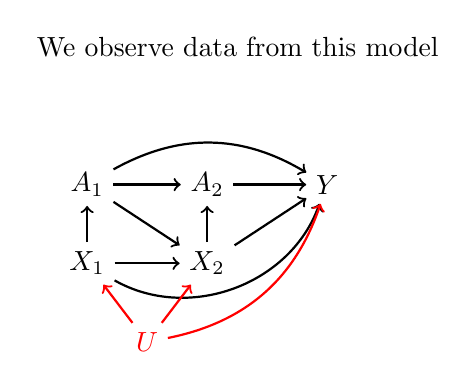
\begin{tikzpicture}[x = .6in]
\node[anchor = north west] at (-.5,2) {We observe data from this model};
\node (y) at (2,0) {$Y$};
\node[red] (u) at (.5,-2) {$U$};
\node (l0) at (0,-1) {$X_1$};
\node (a0) at (0,0) {$A_1$};
\node (l1) at (1,-1) {$X_2$};
\draw[->, thick] (l0) -- (a0);
\draw[->, thick] (l0) to[bend right = 50] (y);
\draw[->, thick] (a0) to[bend left] (y);
\node (a1) at (1,0) {$A_2$};
\draw[->, thick] (a0) -- (a1);
\draw[->, thick] (l0) -- (l1);
\draw[->, thick] (a0) -- (l1);
\draw[->, thick] (l1) -- (a1);
\draw[->, thick] (l1) -- (y);
\draw[->, thick] (a1) -- (y);
\draw[->, thick, red] (u) -- (l0);
\draw[->, thick, red] (u) -- (l1);
\draw[->, thick, red] (u) to[bend right] (y);
\end{tikzpicture} \pause \qquad 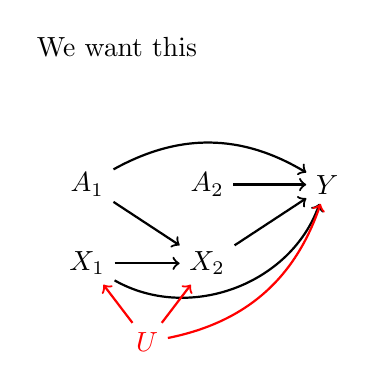
\begin{tikzpicture}[x = .6in]
\node[anchor = north west, align = left] at (-.5,2) {We want this};
\node (y) at (2,0) {$Y$};
\node[red] (u) at (.5,-2) {$U$};
\node (l0) at (0,-1) {$X_1$};
\node (a0) at (0,0) {$A_1$};
\node (l1) at (1,-1) {$X_2$};
%\draw[->, thick, dashed] (l0) -- (a0);
\draw[->, thick] (l0) to[bend right = 50] (y);
\draw[->, thick] (a0) to[bend left] (y);
\node (a1) at (1,0) {$A_2$};
%\draw[->, thick, dashed] (a0) -- (a1);
\draw[->, thick] (l0) -- (l1);
\draw[->, thick] (a0) -- (l1);
%\draw[->, thick, dashed] (l1) -- (a1);
\draw[->, thick] (l1) -- (y);
\draw[->, thick] (a1) -- (y);
\draw[->, thick, red] (u) -- (l0);
\draw[->, thick, red] (u) -- (l1);
\draw[->, thick, red] (u) to[bend right] (y);
\end{tikzpicture}

\end{frame}

\begin{frame}{Inverse probability of treatment weighting}


\begin{tikzpicture}[x = \textwidth, y = .8\textheight]
\node at (0,0) {};
\node at (1,1) {};
\node[anchor = north] at (.45,.9) {$X = 0$};
\node[anchor = north] at (.85,.9) {$X = 1$};
\only<1-3>{
\draw[rounded corners] (.3,.4) rectangle (.6,1);
\draw[rounded corners] (.7,.4) rectangle (1,1);
}
\only<4->{
\draw[dashed, rounded corners] (.3,.4) rectangle (.6,1);
\draw[dashed, rounded corners] (.7,.4) rectangle (1,1);
}
\node[anchor = north west, gray, font = \Huge] (unsamp) at (0,.9) {$\bullet$};
\node[anchor = west, gray] at (unsamp.east) {Untreated};
\node[anchor = north west, blue, font = \Huge] (samp) at (unsamp.south west) {$\bullet$};
\node[anchor = west, blue] (samp.east) at (samp.east) {Treated};
% L = 0
\node[gray, font = \Huge] at (.4,.6) {$\bullet$};
\node[blue, font = \Huge] at (.5,.5) {$\bullet$};
\node[gray, font = \Huge] at (.55,.45) {$\bullet$};
\node[gray, font = \Huge] at (.45,.7) {$\bullet$};
\only<4->{
\node[gray, font = \small, anchor = south, outer sep = 4pt] at (.4,.6) {4/3};
\node[blue, font = \small, anchor = south, outer sep = 4pt] at (.5,.5) {4};
\node[gray, font = \small, anchor = south, outer sep = 4pt] at (.55,.45) {4/3};
\node[gray, font = \small, anchor = south, outer sep = 4pt] at (.45,.7) {4/3};
}
% L = 1
\node[blue, font = \Huge] at (.75,.52) {$\bullet$};
\node[blue, font = \Huge] at (.85,.44) {$\bullet$};
\node[blue, font = \Huge] at (.95,.63) {$\bullet$};
\node[gray, font = \Huge] at (.9,.72) {$\bullet$};
\only<4->{
\node[blue, font = \small, anchor = south, outer sep = 4pt] at (.75,.52) {4/3};
\node[blue, font = \small, anchor = south, outer sep = 4pt] at (.85,.44) {4/3};
\node[blue, font = \small, anchor = south, outer sep = 4pt] at (.95,.63) {4/3};
\node[gray, font = \small, anchor = south, outer sep = 4pt] at (.9,.72) {4};
}
% P(S)
\node<2->[anchor = east, font = \large] at (.45,.2) {Propensity score:};
\node<2->[anchor = west, font = \large] at (.5,.2) {$\pi_i = \P(A = A_i\mid X = X_i)$};
\node<3->[anchor = east, font = \large] at (.45,.1) {Inverse probability weight:};
\node<3->[anchor = west, font = \large] at (.5,.1) {$w_i = \frac{1}{\pi_i}$};
\only<5->{
\node[anchor = west, align = left, font = \footnotesize] at (0.01,.6) {pseudo-population};
\node[font = \small] (l) at (.03,.5) {$L$};
\node[font = \small] (a) at (.13,.5) {$A$};
\node[font = \small] (y) at (.23,.5) {$Y$};
\draw[->, thick] (a) -- (y);
\draw[->, thick] (l) to[bend left] (y);
\draw[dashed, rounded corners] (.01,.45) rectangle (.27,.65);
}
\end{tikzpicture}

\end{frame}

\begin{frame}{Inverse probability weighting}

At every time $t$, define an inverse probability of treatment weight\\
given the measured past confounders and treatments
$$W^{A_t} = \frac{1}{\P(A_t\mid \bar{A}_{t-1}, \bar{L}_t)}$$ \vskip .3in \pause
Define the overall weight as the product
$$W^{\bar{A}} = \prod_{k=1}^K \frac{1}{\P(A_k\mid \bar{A}_{k-1},\bar{L}_k)}$$

\end{frame}

\begin{frame}{Inverse probability weighting}
The weight
$$W^{\bar{A}} = \prod_{k=1}^K \frac{1}{\P(A_k\mid \bar{A}_{k-1},\bar{L}_k)}$$ \vskip .2in
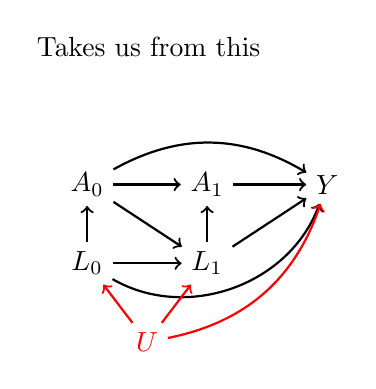
\begin{tikzpicture}[x = .6in]
\node[anchor = north west] at (-.5,2) {Takes us from this};
\node (y) at (2,0) {$Y$};
\node[red] (u) at (.5,-2) {$U$};
\node (l0) at (0,-1) {$L_0$};
\node (a0) at (0,0) {$A_0$};
\node (l1) at (1,-1) {$L_1$};
\draw[->, thick] (l0) -- (a0);
\draw[->, thick] (l0) to[bend right = 50] (y);
\draw[->, thick] (a0) to[bend left] (y);
\node (a1) at (1,0) {$A_1$};
\draw[->, thick] (a0) -- (a1);
\draw[->, thick] (l0) -- (l1);
\draw[->, thick] (a0) -- (l1);
\draw[->, thick] (l1) -- (a1);
\draw[->, thick] (l1) -- (y);
\draw[->, thick] (a1) -- (y);
\draw[->, thick, red] (u) -- (l0);
\draw[->, thick, red] (u) -- (l1);
\draw[->, thick, red] (u) to[bend right] (y);
\end{tikzpicture}  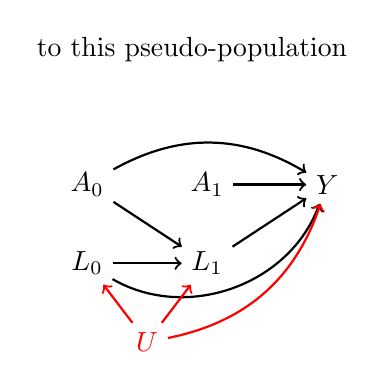
\begin{tikzpicture}[x = .6in]
\node[anchor = north west, align = left] at (-.5,2) {to this pseudo-population};
\node (y) at (2,0) {$Y$};
\node[red] (u) at (.5,-2) {$U$};
\node (l0) at (0,-1) {$L_0$};
\node (a0) at (0,0) {$A_0$};
\node (l1) at (1,-1) {$L_1$}; 
%\draw[->, thick, dashed] (l0) -- (a0);
\draw[->, thick] (l0) to[bend right = 50] (y);
\draw[->, thick] (a0) to[bend left] (y);
\node (a1) at (1,0) {$A_1$};
%\draw[->, thick, dashed] (a0) -- (a1);
\draw[->, thick] (l0) -- (l1);
\draw[->, thick] (a0) -- (l1);
%\draw[->, thick, dashed] (l1) -- (a1);
\draw[->, thick] (l1) -- (y);
\draw[->, thick] (a1) -- (y);
\draw[->, thick, red] (u) -- (l0);
\draw[->, thick, red] (u) -- (l1);
\draw[->, thick, red] (u) to[bend right] (y);
\end{tikzpicture}
\end{frame}

\begin{frame}{Marginal structural models}

\begin{itemize}
\item inverse probability weighting estimates by weighted means
$$\E(Y^{a_1=1,a_2=1}) = \frac{1}{\sum_{i:\vec{A}=1}w_i}\sum_{i:\vec{A}=1}Y_iw_i$$
\item marginal structural model estimates by a weighted regression 
$$\E(Y^{a_1,a_2}) = \beta_0 + \beta_1 a_1 + \beta_2 a_2$$
%where this example gains efficiency by excluding the interaction
\end{itemize}

\end{frame}

\begin{frame}{Let's try it}

\begin{itemize}
\item logistic regression for treatment at each time
\item predict the propensity score
\item create inverse probability weights
\item estimate by IPW and MSM
\end{itemize}

\vskip .15in
\begin{center}
\begin{tabular}{ccc}
A1 & A2 & estimate \\
\hline
0 & 0 & $\hat\E(Y^{00})$ \\
0 & 1 & $\hat\E(Y^{01})$ \\
1 & 0 & $\hat\E(Y^{10})$ \\
1 & 1 & $\hat\E(Y^{11})$
\end{tabular}
\end{center}

\end{frame}

\begin{frame}
\centering
\includegraphics[height = .8\textheight]{figures/msm_samples}
\end{frame}

\begin{frame}
\centering
\includegraphics[height = .8\textheight]{figures/msm_variance}
\end{frame}

\end{document}